\documentclass[conference]{IEEEtran}
\IEEEoverridecommandlockouts

\usepackage{cite}
\usepackage{amsmath,amssymb,amsfonts}
\usepackage{algorithmic}
\usepackage{graphicx}
\usepackage{textcomp}
\usepackage{xcolor}
\usepackage{booktabs}
\usepackage{multirow}
\usepackage{url}
\usepackage{hyperref}

\hypersetup{
    colorlinks=true,
    linkcolor=black,
    citecolor=black,
    urlcolor=black
}

\def\BibTeX{{\rm B\kern-.05em{\sc i\kern-.025em b}\kern-.08em
    T\kern-.1667em\lower.7ex\hbox{E}\kern-.125emX}}

\begin{document}

\title{Context-Aware Document-Level Neural Machine Translation for Indian Languages Using Semantic Retrieval and Gated Context Fusion}

% Note on Faculty Guide Attribution:
% Dr. G. Narayana is explicitly designated as "(Project Guide)" to clarify his supervisory role
% and avoid incorrectly implying co-authorship without prior confirmation.
\author{
\IEEEauthorblockN{Durki Poshanna\IEEEauthorrefmark{1}, G. Vamshi Krishna\IEEEauthorrefmark{1}, and Dr. G. Narayana\IEEEauthorrefmark{2} (Project Guide)}
\IEEEauthorblockA{\IEEEauthorrefmark{1}Department of Artificial Intelligence and Machine Learning\\
Chaitanya Bharathi Institute of Technology (CBIT), Hyderabad, India\\
Roll / Reg. No.: [Roll No. -- Durki Poshanna], [Roll No. -- G. Vamshi Krishna]\\
Email: [Email -- Durki Poshanna], [Email -- G. Vamshi Krishna]}
\IEEEauthorblockA{\IEEEauthorrefmark{2}Project Guide, [Designation / Academic Title (e.g., Associate Professor)], Department of Artificial Intelligence and Machine Learning\\
Chaitanya Bharathi Institute of Technology (CBIT), Hyderabad, India\\
Email: [Email -- Dr. G. Narayana]}
}

\maketitle

\begin{abstract}
Sentence-level Neural Machine Translation (NMT) models process sentences independently, disregarding vital cross-sentence discourse context, inter-sentential pronoun resolution, and lexical cohesion. This limitation is particularly pronounced when translating into morphologically rich, resource-constrained Indian languages such as Telugu. Although massively multilingual foundation models like NLLB-200 demonstrate strong lexical coverage, fine-tuning their entire parameter space on document-level objectives is computationally prohibitive and susceptible to catastrophic forgetting. 

In this work, we investigate a lightweight, parameter-efficient gated context-fusion framework that augments a frozen sentence-level NLLB-200 backbone ($600\text{M}$ parameters) with causal document-level conditioning. Rather than altering the underlying sequence-to-sequence backbone into a native document-level architecture or directly modifying internal decoder layers, our approach introduces an encoder-side Context Adapter. Contextual sentences from preceding document history are semantically retrieved using a frozen MiniLM sentence encoder and projected into the translation model's hidden dimension. A learned gating mechanism, initialized near zero to prevent representation distortion, dynamically modulates the integration of context representations into the NLLB encoder hidden states before decoder cross-attention. 

We evaluate our method on an audited, document-grounded English--Telugu parallel corpus derived from DocHPLT. Preliminary empirical findings on a 100-example validation subset indicate that training the Context Adapter ($2,494,464$ trainable parameters; 0.4\% of backbone capacity) for a single epoch over 1,000 parallel pairs improves validation translation quality over the frozen sentence-level baseline from 7.35 to 13.99 BLEU (+6.64 absolute) and from 25.11 to 31.94 chrF++ (+6.83 absolute). In a separate 12-example diagnostic evaluation, our gated adapter circumvents the catastrophic degradation observed with naive text prefix concatenation, which suffers a 31.06 BLEU drop. We conduct per-example error analyses highlighting both disambiguation improvements and failure cases involving copy interference, providing focused preliminary benchmarks without claiming statistical significance or broad generalization.
\end{abstract}

\begin{IEEEkeywords}
Neural Machine Translation, Document-Level Translation, Indian Languages, Semantic Retrieval, Gated Context Fusion, Context Adapter, NLLB-200, Telugu.
\end{IEEEkeywords}

\section{Introduction}
\label{sec:intro}

Neural Machine Translation (NMT) has achieved remarkable progress across diverse global language pairs \cite{vaswani2017attention, costajussa2022nllb}. However, the prevailing paradigm remains strictly sentence-level: translation models map isolated source sentences into target sentences under the independent and identically distributed assumption. In real-world documents, human communication relies heavily on discourse phenomena such as inter-sentential anaphora, honorific agreement, elliptical omission, and topic-driven lexical consistency \cite{voita-etal-2018-context, voita-etal-2019-good, maruf-etal-2021-survey}. Translating sentences in isolation frequently yields grammatically valid but contextually erroneous translations, where gender markers shift arbitrarily between adjacent lines, entities lose referential coherence, and polysemous terms fluctuate inconsistently across paragraphs \cite{bawden-etal-2018-evaluating}.

These discourse challenges are exacerbated in Dravidian and Indo-Aryan languages of the Indian subcontinent, such as Telugu, Hindi, and Tamil \cite{ramesh-etal-2022-samanantar, gala2023indictrans}. Telugu is an agglutinative language characterized by rich verbal morphology, postpositional inflection, overt gender-number-person agreement, and distinct honorific registers that depend intrinsically on preceding discourse participants. When translating from English (a language with analytic morphology and Subject-Verb-Object word order) into Telugu (Subject-Object-Verb word order with extensive nominal compounding), sentence-level models frequently fail to disambiguate third-person pronouns (e.g., English ``he''/``she'' mapping to polite ``\textit{aayana}''/``\textit{aame}'' versus informal ``\textit{vadu}''/``\textit{aame}'') or maintain specialized domain terminology across consecutive sentences.

Massively multilingual foundation models, notably Meta's NLLB-200 \cite{costajussa2022nllb}, provide unprecedented pretraining representations across more than 200 languages. Nonetheless, NLLB-200 was pretrained almost entirely on isolated sentences mined from the web. Directly fine-tuning all 600 million parameters of NLLB-200 on document-level objectives poses severe obstacles:
\begin{enumerate}
    \item \textbf{Resource Scarcity:} Document-aligned bilingual corpora for Indian languages are sparse; widely used datasets like Samanantar \cite{ramesh-etal-2022-samanantar} are mined as sentence-level pairs lacking document boundaries.
    \item \textbf{Computational Burden:} Full parameter updating requires high-end accelerator clusters that are inaccessible to many academic laboratories.
    \item \textbf{Catastrophic Degradation:} Naive text-level conditioning (prepending preceding context sentences into the source string) severely degrades generation on sentence-level pretrained backbones, triggering repetition loops and catastrophic lexical copying \cite{kim-etal-2019-document}.
\end{enumerate}

To overcome these barriers without altering or updating the underlying translation backbone, we present a parameter-efficient, context-aware translation architecture based on \textit{semantic retrieval} and \textit{gated context fusion}. Rather than treating all preceding document sentences as equally relevant or appending raw text prefixes, our system employs a sentence embedding model (\texttt{all-MiniLM-L6-v2}) \cite{reimers-gurevych-2019-sentence, wang2020minilm} to semantically score and retrieve the most salient prior sentences from the source document. A lightweight Context Adapter ($2,494,464$ parameters) projects the context representation into the hidden space of NLLB-200 and employs a learned gating residual mechanism to fuse the contextual information directly into the encoder hidden states before cross-attention decoding. Rather than modifying internal decoder layers or converting the system into a native document-level architecture, this modular design allows the frozen decoder to attend to contextually conditioned encoder representations. Crucially, the gate bias is initialized negatively, ensuring that prior to training, the model defaults to the reliable sentence-level baseline representation.

Our experimental study, conducted on an audited English--Telugu document parallel corpus extracted from DocHPLT \cite{obrien2025dochplt}, investigates three central research questions:
\begin{itemize}
    \item \textbf{RQ1:} Can a lightweight, frozen-backbone Context Adapter improve document-level translation quality into low-resource Indian languages without updating backbone weights?
    \item \textbf{RQ2:} How does gated representation fusion compare against naive prefix concatenation in frozen multilingual models?
    \item \textbf{RQ3:} How sensitive is translation performance to context window depth and semantic retrieval scoring?
\end{itemize}

\noindent\textbf{Key Contributions of this work:}
\begin{enumerate}
    \item We design and implement a parameter-efficient encoder-side Context Adapter architecture with learned gating that fuses dense semantic context into frozen multilingual NMT encoder hidden states before cross-attention decoding, without modifying decoder layers or converting the model into a native document-level architecture ($2.49\text{M}$ trainable parameters, 0.4\% of backbone capacity).
    \item We report preliminary empirical findings on an audited 100-example English--Telugu validation subset from DocHPLT, demonstrating that the adapter improves translation quality over the frozen sentence-level baseline from 7.35 to 13.99 BLEU (+6.64 absolute) and from 25.11 to 31.94 chrF++ (+6.83 absolute). In a separate 12-example diagnostic evaluation, we verify that gated fusion circumvents the severe degradation (-31.06 BLEU) observed with naive prefix concatenation.
    \item We conduct a rigorous per-example diagnostic and error analysis on the validation subset, detailing both contextual disambiguation improvements and concrete failure modes (such as copy interference), establishing a transparent preliminary baseline without asserting statistical significance or broad cross-lingual generalization.
\end{enumerate}

\section{Related Work}
\label{sec:related_work}

\subsection{Machine Translation for Indian Languages}
Neural machine translation for Indian languages has developed rapidly through large-scale data aggregation and multilingual pretraining. The AI4Bharat Samanantar corpus \cite{ramesh-etal-2022-samanantar} contributed 49.7 million sentence pairs across 11 Indic languages, catalyzing foundational models such as IndicTrans2 \cite{gala2023indictrans}. Concurrently, NLLB-200 \cite{costajussa2022nllb} scaled translation across 200 languages, establishing strong baselines for low-resource pairs. However, existing parallel resources for Indian languages are predominantly sentence-level. Even when mined from web texts, sentence pairs in corpora like Samanantar undergo deduplication and shuffling, stripping document context and paragraph boundaries. The recent release of DocHPLT \cite{obrien2025dochplt} offers an authentic, document-aligned bilingual corpus mined with web-scale document preservation, enabling principled document-level NMT research in Indian languages.

\subsection{Document-Level Neural Machine Translation}
Research in document-level NMT has explored multiple architectural paradigms \cite{maruf-etal-2021-survey}. Early strategies explored multi-encoder architectures \cite{jean2017does, voita-etal-2018-context, zhang-etal-2018-improving}, where separate Transformer encoders process the current sentence and neighboring context sentences before fusing them via cross-attention or gating. Hierarchical attention networks \cite{miculicich-etal-2018-document} model discourse structure across sentence and document levels. Memory-augmented networks \cite{maruf-haffari-2018-document} and continuous cache architectures \cite{tu-etal-2018-learning} store past translation states for dynamic retrieval during decoding.

An alternative line of inquiry investigates concatenation models (extended context) \cite{tiedemann-scherrer-2017-neural, ma-etal-2020-simple}, where consecutive sentences are concatenated into a single input sequence separated by special tokens. While concatenation models can learn discourse relationships when trained end-to-end on massive document corpora, studies by Kim et al. \cite{kim-etal-2019-document} and Fernandes et al. \cite{fernandes-etal-2021-measuring} revealed that when applied to frozen or sentence-pretrained models, concatenation often suffers from context neglect, sequence truncation, and erratic copy behavior. Our work addresses this limitation by injecting dense, semantically retrieved context representations through a controlled gating interface.

\subsection{Parameter-Efficient Fine-Tuning and Adapters}
Parameter-efficient fine-tuning (PEFT) has emerged as the standard paradigm for adapting large pretrained models without the computational overhead of full fine-tuning \cite{houlsby2019parameter}. In NMT, Bapna and Firat \cite{bapna-firat-2019-simple} demonstrated that lightweight residual adapter modules inserted between frozen Transformer layers enable modular domain adaptation. Unlike conventional bottleneck adapters that modify intra-layer representations across all Transformer blocks, our Context Adapter specifically targets the interface between the source sentence representation and the decoder cross-attention, using a single projection and gate module to incorporate document context.

\subsection{Discourse Evaluation and Benchmarks}
Standard lexical overlap metrics such as BLEU \cite{post-2018-call} and chrF++ \cite{popovic-2017-chrf} compute n-gram matches at the corpus level, but often show limited sensitivity to nuanced discourse phenomena \cite{bawden-etal-2018-evaluating}. Targeted contrastive test sets, such as ContraPro for German pronoun translation \cite{muller2018large} and the discourse datasets introduced by Voita et al. \cite{voita-etal-2019-good}, have highlighted that minor BLEU differences may obscure substantial gains in pronominal consistency and cohesion. In Indian languages, formal discourse challenge suites remain nascent; consequently, researchers must pair automated corpus metrics with granular sentence-level diagnostics and manual review.

\section{Research Gap and Problem Formulation}
\label{sec:gap}

Despite advances in multilingual NMT, a clear gap persists at the intersection of document-level discourse modeling, parameter-efficient adaptation, and Indian languages:
\begin{enumerate}
    \item \textbf{The Frozen-Backbone Dilemma:} State-of-the-art multilingual models like NLLB-200 cannot be practically fine-tuned end-to-end in resource-constrained environments, yet naive prompt/prefix conditioning triggers severe performance degradation.
    \item \textbf{Absence of Context Selection:} Prior concatenation methods blindly absorb adjacent lines regardless of topical relatedness, introducing irrelevant tokens into the limited context window.
    \item \textbf{Resource Constraints for Indic Documents:} No prior study has systematically evaluated gated context adapters on strictly aligned English--Telugu document corpora while maintaining strict data provenance.
\end{enumerate}

To bridge this gap, we formulate context-aware translation as follows: Given a source document consisting of ordered sentences $\mathcal{D} = (S_1, S_2, \dots, S_N)$, the task is to translate a target sentence $S_t = (x_1, \dots, x_L)$ at position $t$ into a target language sentence $Y_t = (y_1, \dots, y_M)$ conditioned on both $S_t$ and the causal document history $\mathcal{C}_t = \{S_1, \dots, S_{t-1}\}$.

\begin{figure*}[t]
\centering
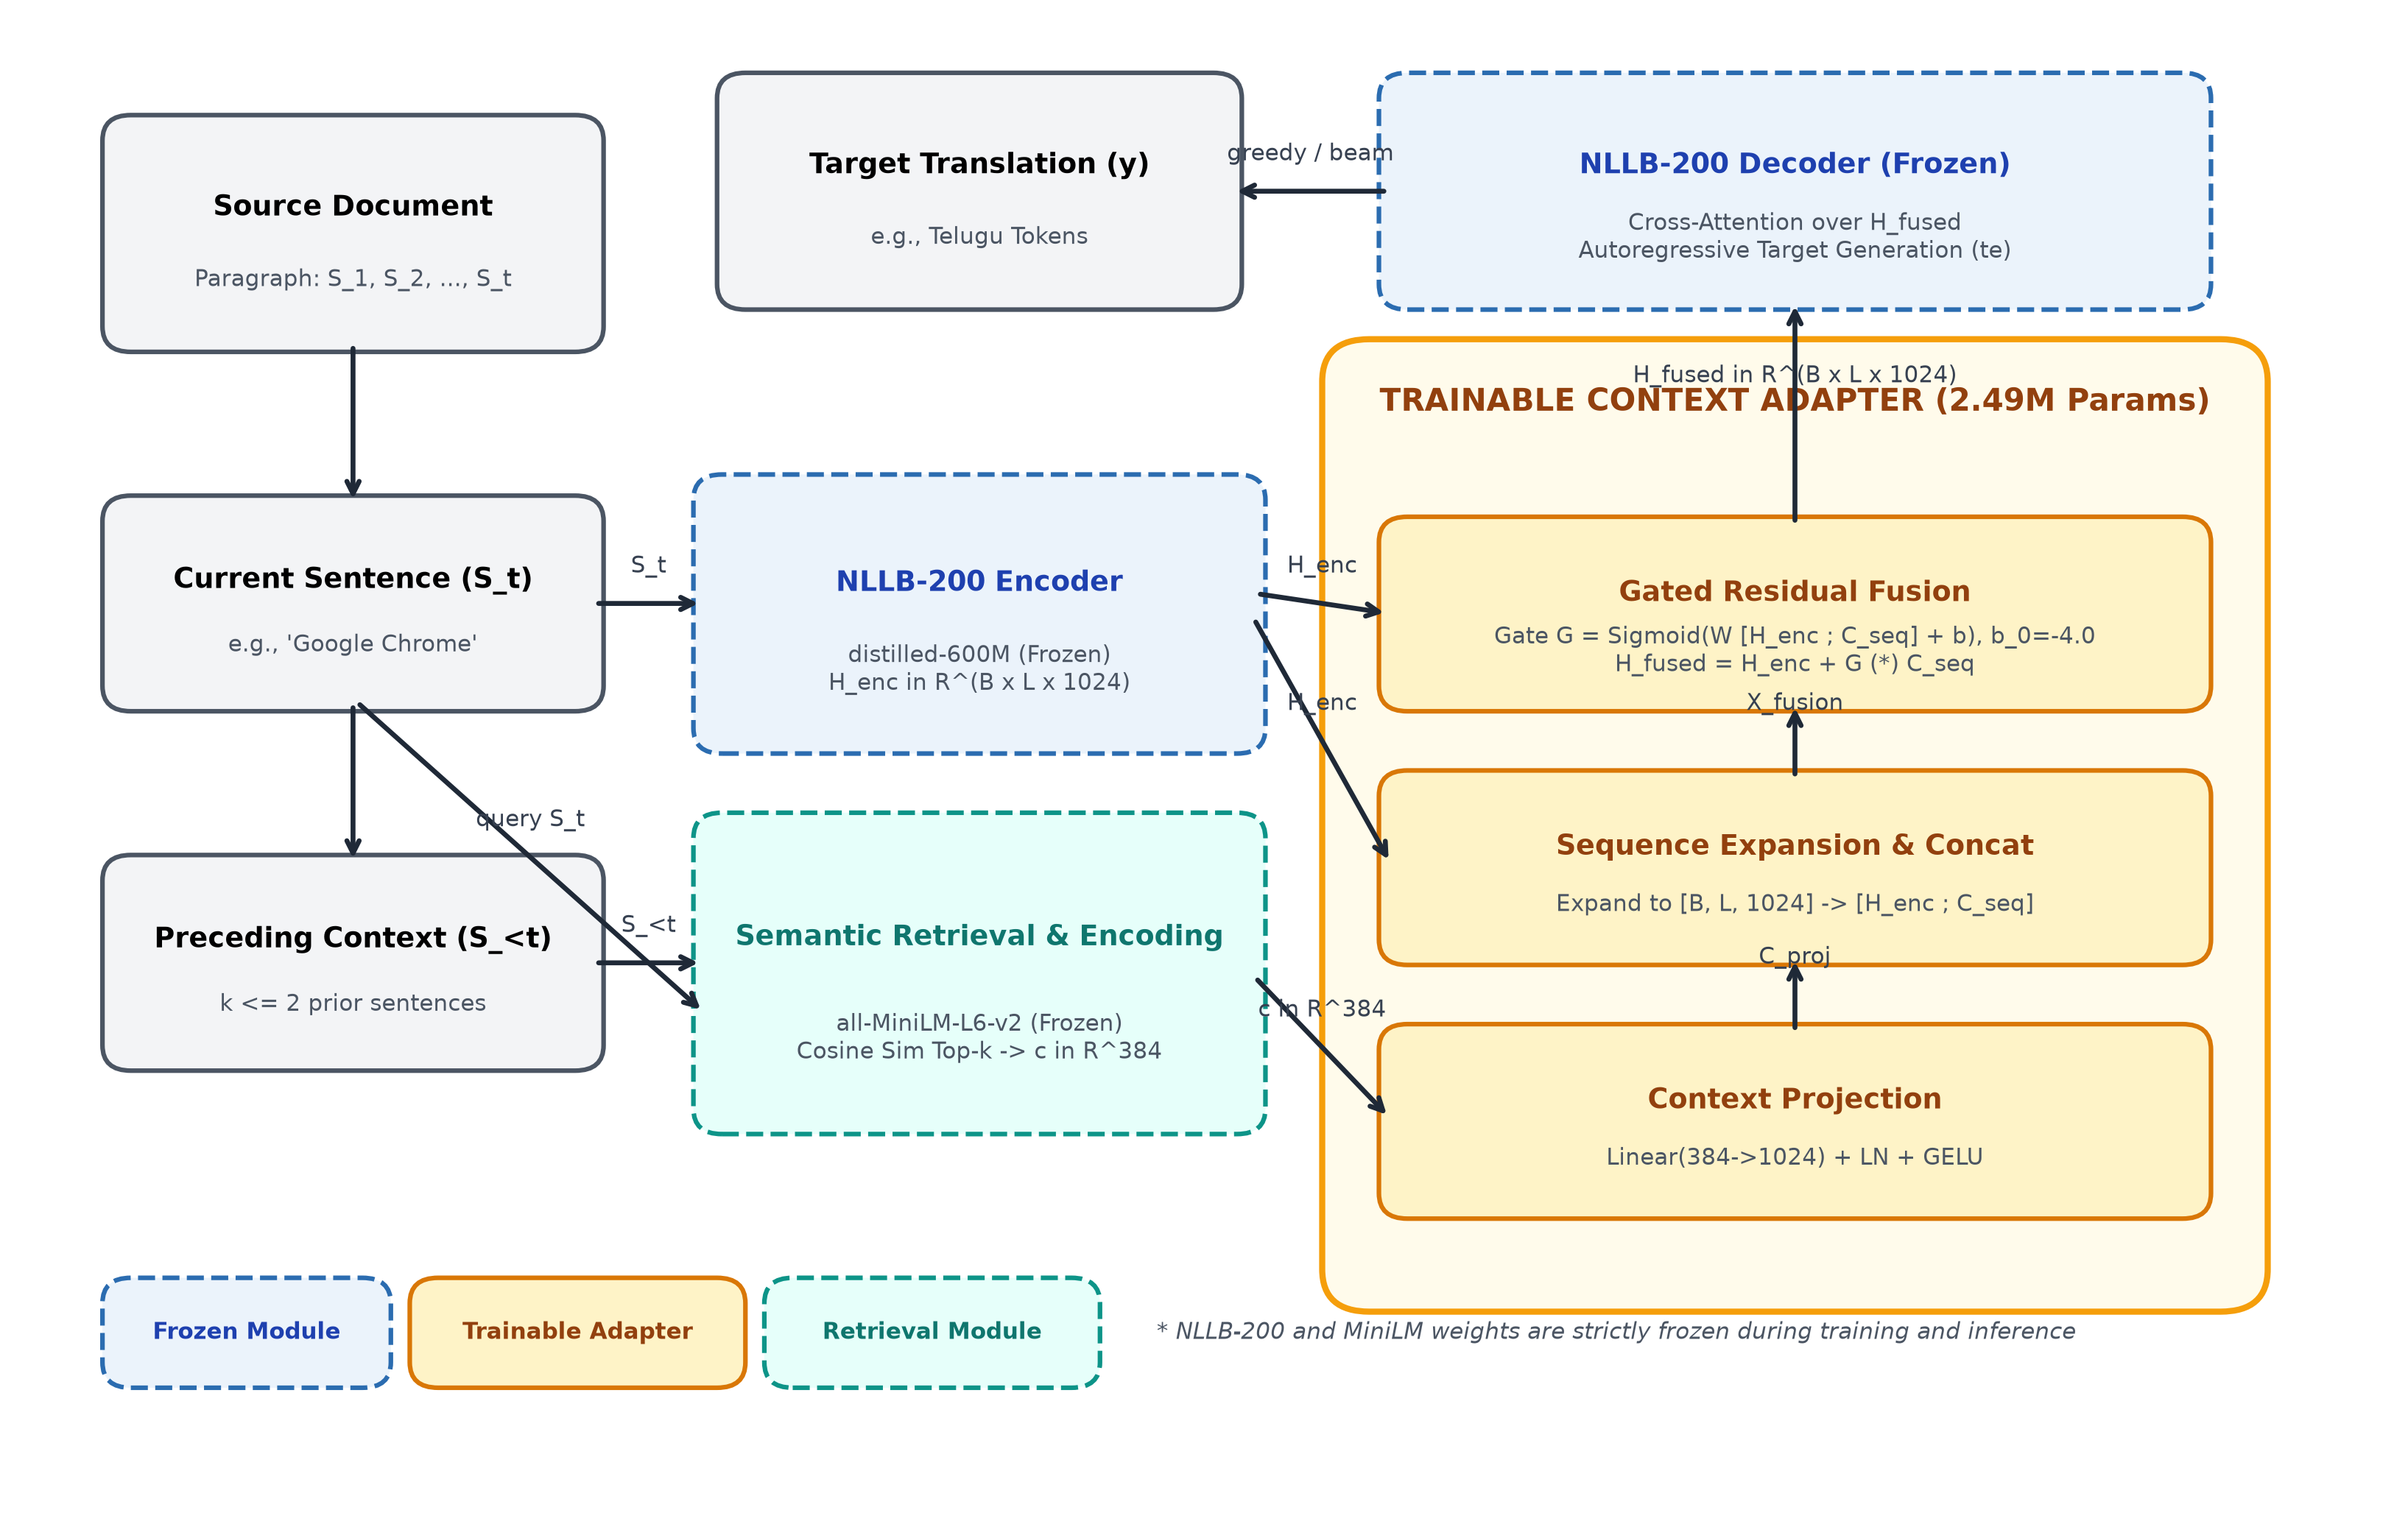
\includegraphics[width=0.92\textwidth]{figures/system_architecture.png}
\caption{System architecture of the proposed Context-Aware Translation framework. A frozen sentence-level NLLB-200 encoder generates source token representations $H_{enc} \in \mathbb{R}^{B \times L \times 1024}$. Concurrently, preceding document sentences $S_{<t}$ are ranked via cosine similarity against $S_t$ using frozen all-MiniLM-L6-v2 embeddings to extract context vector $c \in \mathbb{R}^{384}$. The trainable Context Adapter ($2.49\text{M}$ parameters) projects $c$ to dimension $1024$, concatenates it with $H_{enc}$, and computes a learned gate $G \in [0, 1]^{B \times L \times 1024}$ initialized to near zero ($b_0 = -4.0$). The resulting fused representation $H_{fused}$ drives the frozen NLLB-200 decoder.}
\label{fig:architecture}
\end{figure*}

\section{Proposed Methodology}
\label{sec:methodology}

The complete pipeline consists of four modular stages: (1) Causal Context Formation, (2) Semantic Context Retrieval and Encoding, (3) Trainable Context Adapter with Gated Fusion, and (4) Autoregressive Translation Generation. Figure~\ref{fig:architecture} illustrates the architectural workflow. Crucially, our system does not constitute a native document-level NMT architecture, nor does it alter or inject representations directly into internal decoder layers. Instead, the projected context is fused exclusively with the frozen NLLB encoder hidden states, providing context-conditioned representations that the frozen decoder attends to via its standard cross-attention mechanism.

\subsection{Causal Context Formation}
To eliminate lookahead bias and future-sentence leakage, context retrieval is strictly causal. For any source sentence $S_t$ in document $\mathcal{D}$, the candidate context set is bounded by:
\begin{equation}
\mathcal{C}_t = \{S_j \in \mathcal{D} \mid 1 \le j < t, \, t - k_{max} \le j \le t - 1\}
\end{equation}
where $k_{max}$ is the maximum historical window size (configured to $k_{max} = 2$ in our primary experiments). If $t = 1$, the context candidate set is empty ($\mathcal{C}_1 = \emptyset$). Crucially, sentence boundaries never cross document borders: candidates are drawn exclusively from the exact source document containing $S_t$.

\subsection{Semantic Context Retrieval and Encoding}
Rather than treating all prior sentences uniformly, we score candidate sentences against $S_t$ using dense semantic representations. We employ the pretrained \texttt{sentence-transformers/all-MiniLM-L6-v2} encoder $E_{ctx}(\cdot)$ \cite{wang2020minilm}, which maps arbitrary text strings into a normalized $d_c = 384$-dimensional embedding space:
\begin{equation}
\mathbf{e}_t = E_{ctx}(S_t) \in \mathbb{R}^{d_c}, \quad \mathbf{e}_j = E_{ctx}(S_j) \in \mathbb{R}^{d_c}
\end{equation}
The semantic relevance score $\text{sim}(S_j, S_t)$ is computed via cosine similarity:
\begin{equation}
\text{sim}(S_j, S_t) = \frac{\mathbf{e}_j \cdot \mathbf{e}_t}{\|\mathbf{e}_j\|_2 \|\mathbf{e}_t\|_2}
\end{equation}
The top-$k$ most similar context sentences are selected:
\begin{equation}
\mathcal{S}^*_t = \operatorname{arg\,top-}k_{S_j \in \mathcal{C}_t} \left(\text{sim}(S_j, S_t)\right)
\end{equation}
The selected context strings are concatenated in chronological order into a unified context text $T_{ctx} = \bigoplus_{S_j \in \mathcal{S}^*_t} S_j$. When $\mathcal{S}^*_t = \emptyset$, $T_{ctx}$ is empty and maps to a zero vector $\mathbf{0} \in \mathbb{R}^{d_c}$. Otherwise, the context embedding vector $c$ is computed as:
\begin{equation}
c = E_{ctx}(T_{ctx}) \in \mathbb{R}^{d_c}
\end{equation}
Throughout training and inference, the parameters of $E_{ctx}(\cdot)$ remain completely frozen.

\subsection{NLLB-200 Source Encoding}
The current sentence $S_t$ is tokenized using the NLLB-200 vocabulary (prefixed with the source language token \texttt{eng\_Latn}) and passed through the frozen NLLB-200 encoder:
\begin{equation}
H_{enc} = \text{Encoder}_{\text{NLLB}}(S_t) \in \mathbb{R}^{B \times L \times d_{model}}
\end{equation}
where $B$ is batch size ($B=1$), $L$ is sequence length ($L \le 128$), and $d_{model} = 1024$ denotes the hidden representation dimension of \texttt{facebook/nllb-200-distilled-600M}.

\subsection{Trainable Context Adapter with Gated Fusion}
The core component of our architecture is the Context Adapter, which maps the $384$-dimensional context embedding into the $1024$-dimensional NLLB encoder space and performs token-wise gated residual fusion with the encoder hidden states before decoder cross-attention.

\subsubsection{Context Projection}
The context vector $c \in \mathbb{R}^{B \times d_c}$ is first projected through a non-linear feed-forward block:
\begin{equation}
c_{proj} = \text{Dropout}\left(\text{GELU}\left(\text{LayerNorm}(W_{p} c + b_p)\right)\right)
\end{equation}
where $W_p \in \mathbb{R}^{d_{model} \times d_c}$ and $b_p \in \mathbb{R}^{d_{model}}$. Dropout is set to $p=0.1$. The projected vector $c_{proj} \in \mathbb{R}^{B \times d_{model}}$ is then unsqueezed and broadcast along the sequence length dimension to match the spatial shape of the encoder states:
\begin{equation}
C_{seq} = \text{broadcast}(c_{proj}, [B, L, d_{model}]) \in \mathbb{R}^{B \times L \times d_{model}}
\end{equation}

\subsubsection{Learned Gating Mechanism}
To determine how strongly each source token should attend to the projected context representation, we compute a sequence-level gate $G \in \mathbb{R}^{B \times L \times d_{model}}$. The encoder hidden states $H_{enc}$ and the context sequence $C_{seq}$ are concatenated along the feature dimension:
\begin{equation}
X_{fusion} = [H_{enc} \,;\, C_{seq}] \in \mathbb{R}^{B \times L \times 2d_{model}}
\end{equation}
The gate is computed via a linear projection followed by an element-wise sigmoid activation:
\begin{equation}
G = \sigma(W_g X_{fusion} + b_g)
\end{equation}
where $W_g \in \mathbb{R}^{d_{model} \times 2d_{model}}$ and $b_g \in \mathbb{R}^{d_{model}}$.

\subsubsection{Near-Zero Gate Initialization}
A frequent failure mode in adapter training is representation shock: randomly initialized adapter weights corrupt the highly optimized representations of the pretrained backbone during early iterations. To ensure smooth training dynamics, we initialize $W_g$ using Xavier uniform initialization, but initialize the gate bias $b_g$ to a constant value of $-4.0$:
\begin{equation}
b_g \leftarrow -4.0 \cdot \mathbf{1} \implies \sigma(b_g) = \frac{1}{1 + e^{4.0}} \approx 0.01798
\end{equation}
At step 0, $G \approx \mathbf{0}$, ensuring that the initial fused representation is virtually identical to the frozen NLLB baseline representation ($H_{fused} \approx H_{enc}$).

\subsubsection{Residual Fusion}
The final fused encoder hidden representation $H_{fused}$ is computed via an element-wise gated residual addition:
\begin{equation}
H_{fused} = H_{enc} + G \odot C_{seq} \in \mathbb{R}^{B \times L \times d_{model}}
\end{equation}
where $\odot$ denotes the Hadamard product.

\subsection{Trainable Parameter Count}
The trainable parameter footprint is derived exactly from the architecture:
\begin{itemize}
    \item \textbf{Linear Projection:} $W_p \in \mathbb{R}^{1024 \times 384}$, $b_p \in \mathbb{R}^{1024}$
    \begin{equation*}
    1024 \times 384 + 1024 = 393,216 + 1,024 = 394,240 \text{ parameters}
    \end{equation*}
    \item \textbf{LayerNorm:} $\gamma, \beta \in \mathbb{R}^{1024}$
    \begin{equation*}
    1024 + 1024 = 2,048 \text{ parameters}
    \end{equation*}
    \item \textbf{Gate Projection:} $W_g \in \mathbb{R}^{1024 \times 2048}$, $b_g \in \mathbb{R}^{1024}$
    \begin{equation*}
    1024 \times 2048 + 1024 = 2,097,152 + 1,024 = 2,098,176 \text{ parameters}
    \end{equation*}
\end{itemize}
\begin{equation}
\Theta_{adapter} = 394,240 + 2,048 + 2,098,176 = 2,494,464 \text{ parameters}
\end{equation}
Compared to the $600\text{M}$ parameters of NLLB-200, the Context Adapter updates only \textbf{0.41\%} of the total network capacity, preserving strict parameter efficiency.

\subsection{Training Procedure}
During adapter training, both the NLLB-200 backbone (encoder and decoder) and the MiniLM context encoder are held completely frozen ($\nabla_{\theta_{NLLB}} = \mathbf{0}, \nabla_{\theta_{MiniLM}} = \mathbf{0}$). Gradients flow exclusively into the Context Adapter parameters $\Theta_{adapter}$.

The target sentence $Y_t = (y_1, \dots, y_M)$ is tokenized with target language prefix \texttt{tel\_Telu}. Cross-entropy loss is computed using native M2M-100 right-shifted decoder inputs:
\begin{equation}
\mathcal{L}(\Theta_{adapter}) = -\sum_{m=1}^M \log P(y_m \mid y_{<m}, H_{fused}; \theta_{NLLB}, \Theta_{adapter})
\end{equation}
Optimization is performed using AdamW with learning rate $\eta = 10^{-4}$, weight decay 0.01, and batch size 1 for 1 epoch (1,000 optimization steps). Training converges smoothly, yielding an average cross-entropy loss of $1.99768$.

\section{Experimental Setup}
\label{sec:experiments}

\subsection{Datasets and Data Provenance}
To ensure reproducibility and eliminate data leakage, we maintain strict data provenance boundaries across all datasets.

\subsubsection{DocHPLT Parallel Corpus}
Document-level experiments are conducted on an audited English--Telugu parallel shard from the DocHPLT corpus \cite{obrien2025dochplt} (shard \texttt{train-00000-of-00030.parquet}, git commit revision \texttt{76a591ec3c014d0ac4193a3cbdfc12689616a8d3}). The audited shard contains 12,996 documents and 118,724 alignment groups. To guarantee unambiguous reference pairs and prevent artificial noise from multi-sentence aggregations, we filter the shard under the following verified criteria:
\begin{itemize}
    \item Strict 1-to-1 sentence alignments only (rejecting 1-to-many, many-to-1, and many-to-many matches).
    \item Bilingual sentence aligner confidence score $\ge 0.70$.
    \item Preserved source document boundaries: each candidate must possess at least one authentic preceding sentence within the same source document. Context is never inferred from row adjacency in the Parquet file.
\end{itemize}
From this clean candidate pool, deterministic sampling (seed 42) creates 1,000 training examples and 100 validation examples.

\subsubsection{Samanantar Baseline Corpus}
As an external sentence-level reference, we also process the AI4Bharat Samanantar English--Telugu corpus \cite{ramesh-etal-2022-samanantar} (upstream revision \texttt{ead34c5b22a0354d350e7dfdd6aece7df5a48f37}). Preprocessing filtered out 18,192 exact duplicate pairs and 326 length-outlier sentences, yielding 4,927,517 valid pairs partitioned into 80\% train ($3,942,014$), 10\% validation ($492,752$), and 10\% test ($492,751$). Because Samanantar lacks document boundary annotations, adjacent rows do not share discourse relationships. Consequently, Samanantar is utilized strictly for sentence-level baseline validation, preventing false document context construction.

\subsection{Model Configurations and Hyperparameters}
Table~\ref{tab:hyperparams} summarizes the execution configuration across models and environments. Decoding is strictly deterministic across all conditions (greedy search, \texttt{num\_beams=1}, \texttt{do\_sample=False}, \texttt{max\_new\_tokens=128}).

\begin{table}[t]
\caption{Model and Training Configurations}
\label{tab:hyperparams}
\centering
\resizebox{\columnwidth}{!}{%
\begin{tabular}{ll}
\toprule
\textbf{Hyperparameter / Attribute} & \textbf{Value / Specification} \\
\midrule
Translation Backbone & \texttt{facebook/nllb-200-distilled-600M} \\
Backbone Parameters & 600 Million (Frozen) \\
Context Encoder & \texttt{sentence-transformers/all-MiniLM-L6-v2} \\
Encoder Parameters & 22.7 Million (Frozen) \\
Context Dimension ($d_c$) & 384 \\
NLLB Hidden Dimension ($d_{model}$) & 1024 \\
Context Adapter Parameters & 2,494,464 (Trainable, 0.4\%) \\
Optimizer & AdamW ($\beta_1=0.9, \beta_2=0.999$) \\
Learning Rate & $1 \times 10^{-4}$ \\
Adapter Dropout & 0.1 \\
Batch Size & 1 \\
Training Steps & 1,000 (1 epoch) \\
Final Training Loss & 1.99768 \\
Source Max Sequence Length & 128 tokens \\
Target Max Sequence Length & 128 tokens \\
Decoding Strategy & Greedy (\texttt{num\_beams=1}, \texttt{do\_sample=False}) \\
Hardware Environment & Intel CPU Execution (Reproducible Seed 42) \\
\bottomrule
\end{tabular}%
}
\end{table}

\section{Evaluation Metrics}
\label{sec:metrics}

We evaluate translation quality using official corpus-level implementations from SacreBLEU \cite{post-2018-call}:
\begin{itemize}
    \item \textbf{BLEU:} Corpus-level bilingual evaluation understudy. We utilize SacreBLEU with effective-order smoothing for short sequences and \texttt{none} tokenization for Telugu target outputs to avoid destructive subword re-tokenization. The metric is computed over full corpus n-gram counts, avoiding arithmetic sentence averaging.
    \item \textbf{chrF++:} Character n-gram F-score augmented with word n-grams \cite{popovic-2017-chrf}. Parameterized with character order $\beta=2$, character n-gram length 6, and word n-gram length 2 (\texttt{char\_order=6}, \texttt{word\_order=2}, \texttt{beta=2}). chrF++ is especially well-suited for agglutinative Indian languages like Telugu, where morphological variations heavily penalize strict word-level BLEU matching.
\end{itemize}

\section{Results and Analysis}
\label{sec:results}

\subsection{Main Validation Results (100-Example Subset)}
Table~\ref{tab:main_results} presents the preliminary evaluation comparing the sentence-level NLLB-200 baseline against our trained Context Adapter on the 100-example DocHPLT validation subset ($k=2$).

\begin{table}[ht]
\caption{Primary Validation Results on DocHPLT (100 Examples)}
\label{tab:main_results}
\centering
\resizebox{\columnwidth}{!}{%
\begin{tabular}{lcccc}
\toprule
\textbf{Model Pipeline} & \textbf{BLEU} & \textbf{chrF++} & \textbf{$\Delta$ BLEU} & \textbf{$\Delta$ chrF++} \\
\midrule
NLLB Baseline (Frozen) & 7.3497 & 25.1066 & -- & -- \\
\textbf{Context Adapter (Ours)} & \textbf{13.9866} & \textbf{31.9352} & \textbf{+6.6368} & \textbf{+6.8285} \\
\midrule
\textit{Relative Improvement (\%)} & \textit{+90.30\%} & \textit{+27.20\%} & -- & -- \\
\bottomrule
\end{tabular}%
}
\end{table}

On this 100-example validation subset, the proposed Context Adapter achieves an absolute gain of \textbf{+6.64 BLEU} points and \textbf{+6.83 chrF++} points over the baseline. Because the underlying NLLB-200 model weights and decoder remain identical between both runs, this empirical delta is attributable directly to the injected semantic context and gated adapter fusion. We emphasize that these results represent preliminary empirical observations on this specific 100-example validation split rather than claims of statistical significance or broad generalization. Figures~\ref{fig:bleu_comp} and \ref{fig:chrf_comp} illustrate these comparative gains.

\begin{figure}[htbp]
\centering
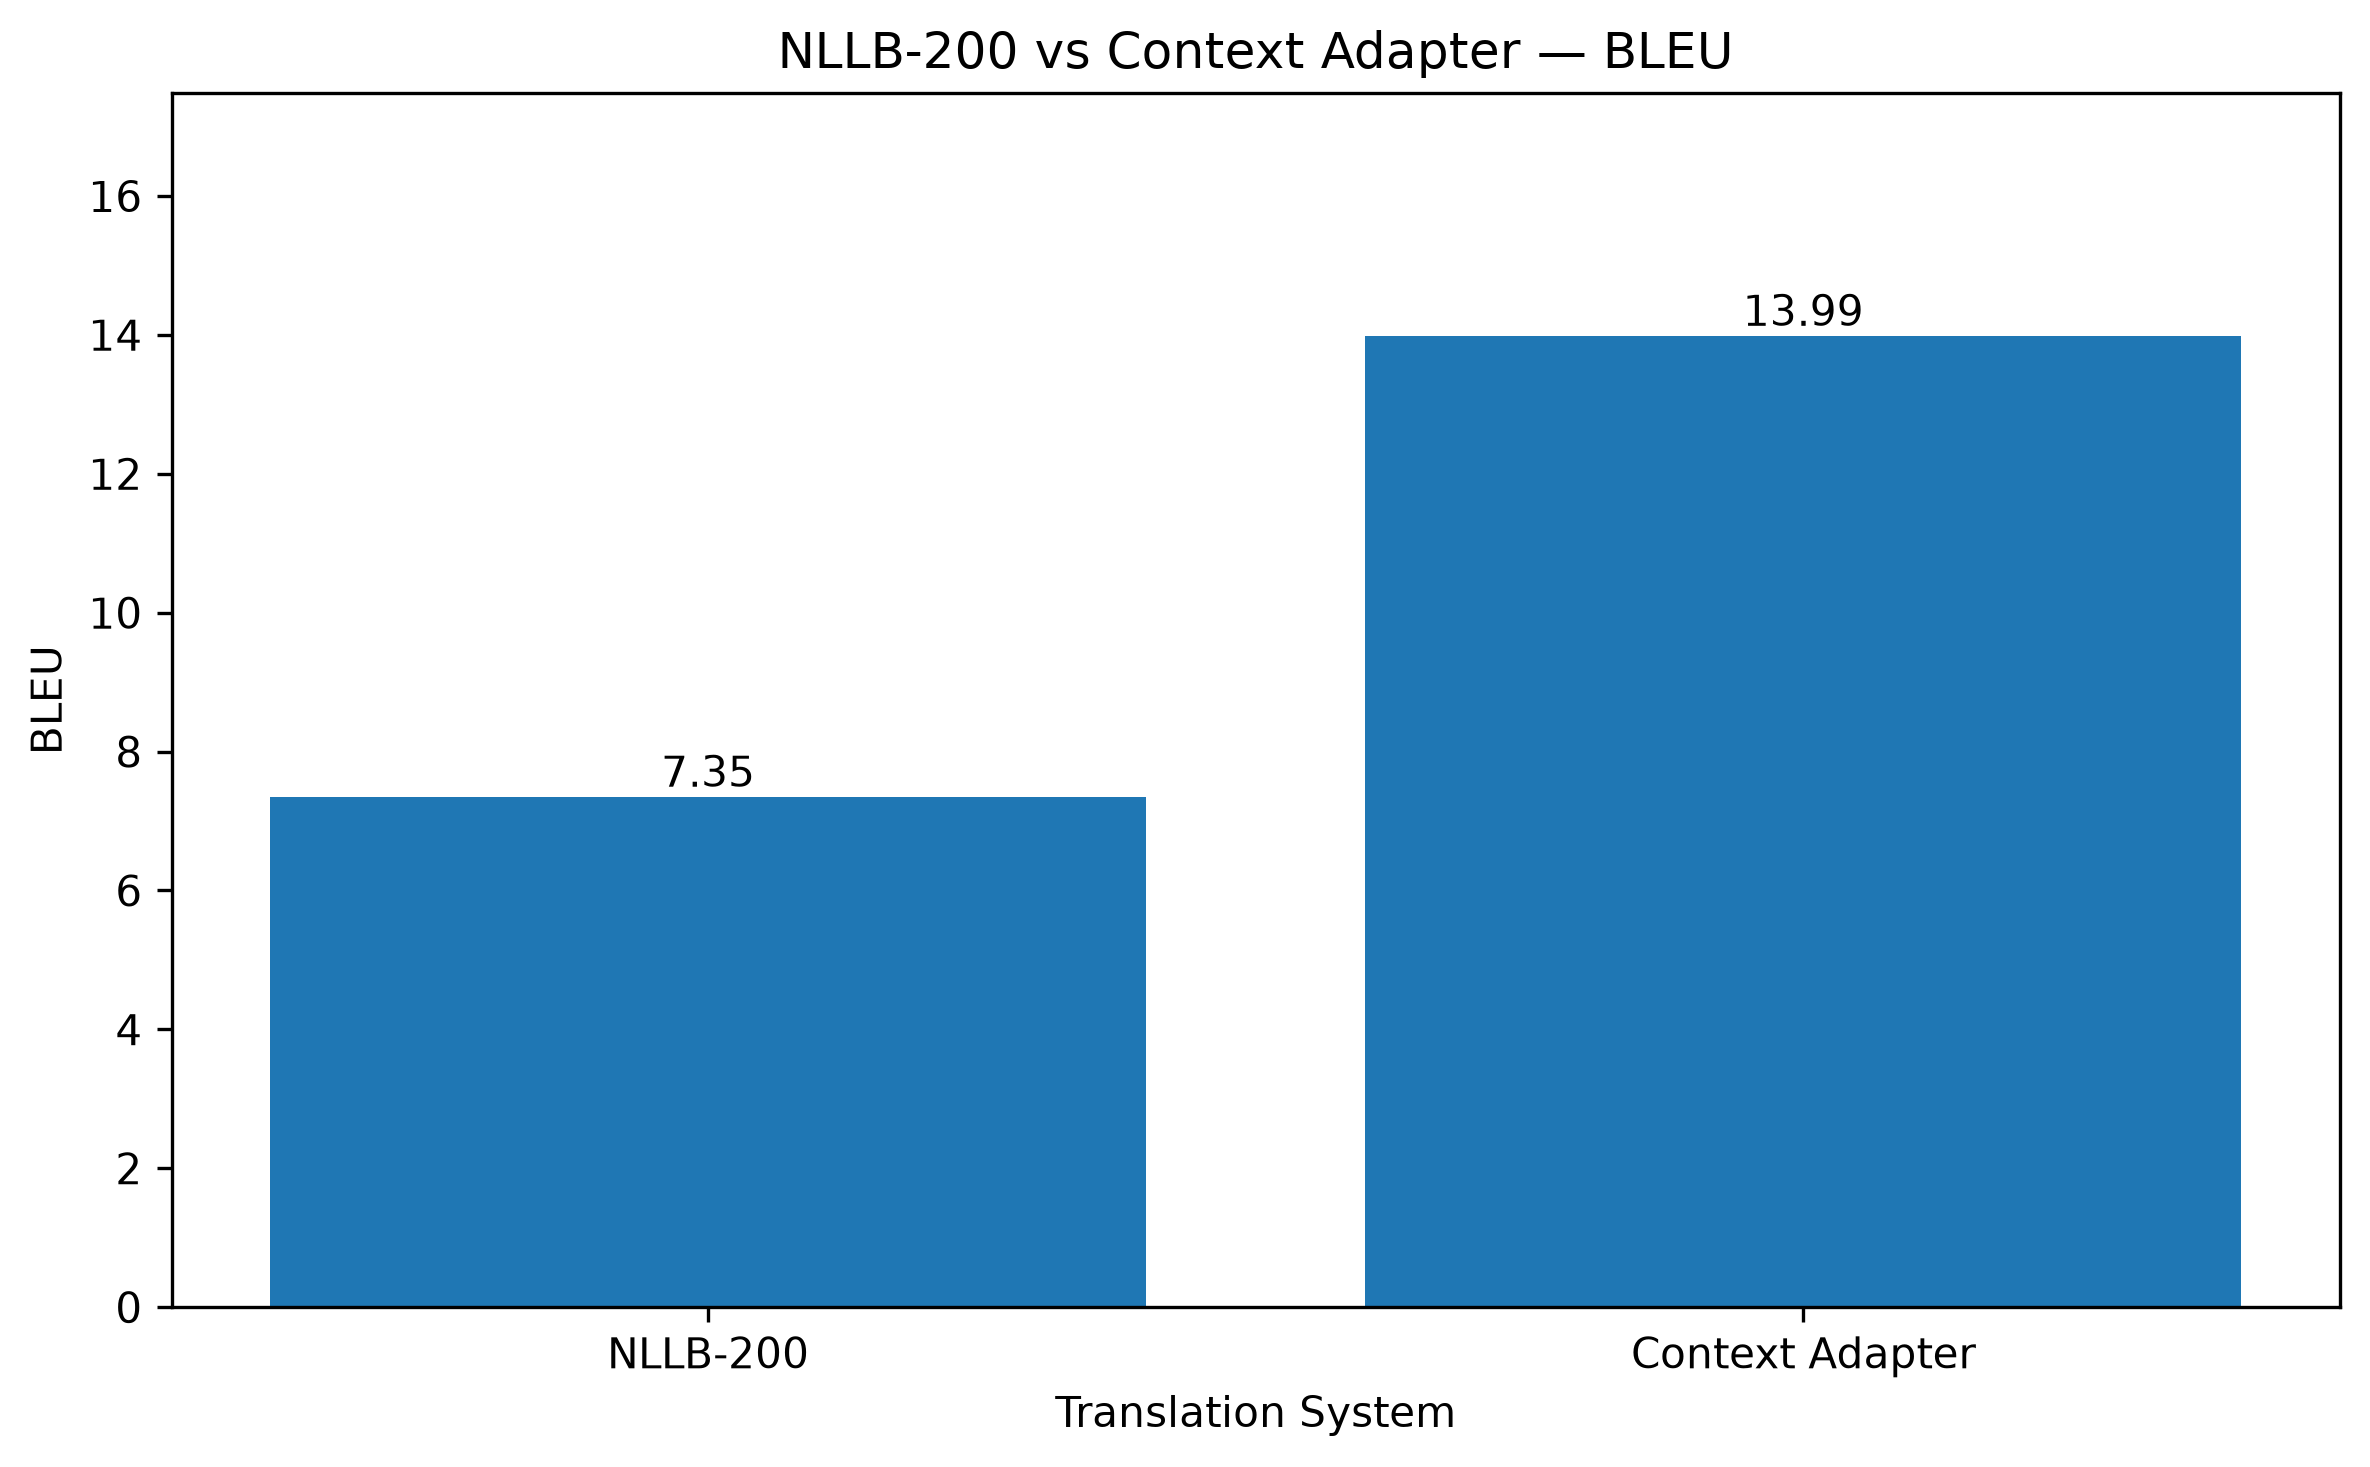
\includegraphics[width=0.82\columnwidth]{figures/final_bleu_comparison.png}
\caption{Corpus BLEU comparison between the frozen sentence-level NLLB-200 baseline and the proposed Context Adapter on the 100-example validation set.}
\label{fig:bleu_comp}
\end{figure}

\begin{figure}[htbp]
\centering
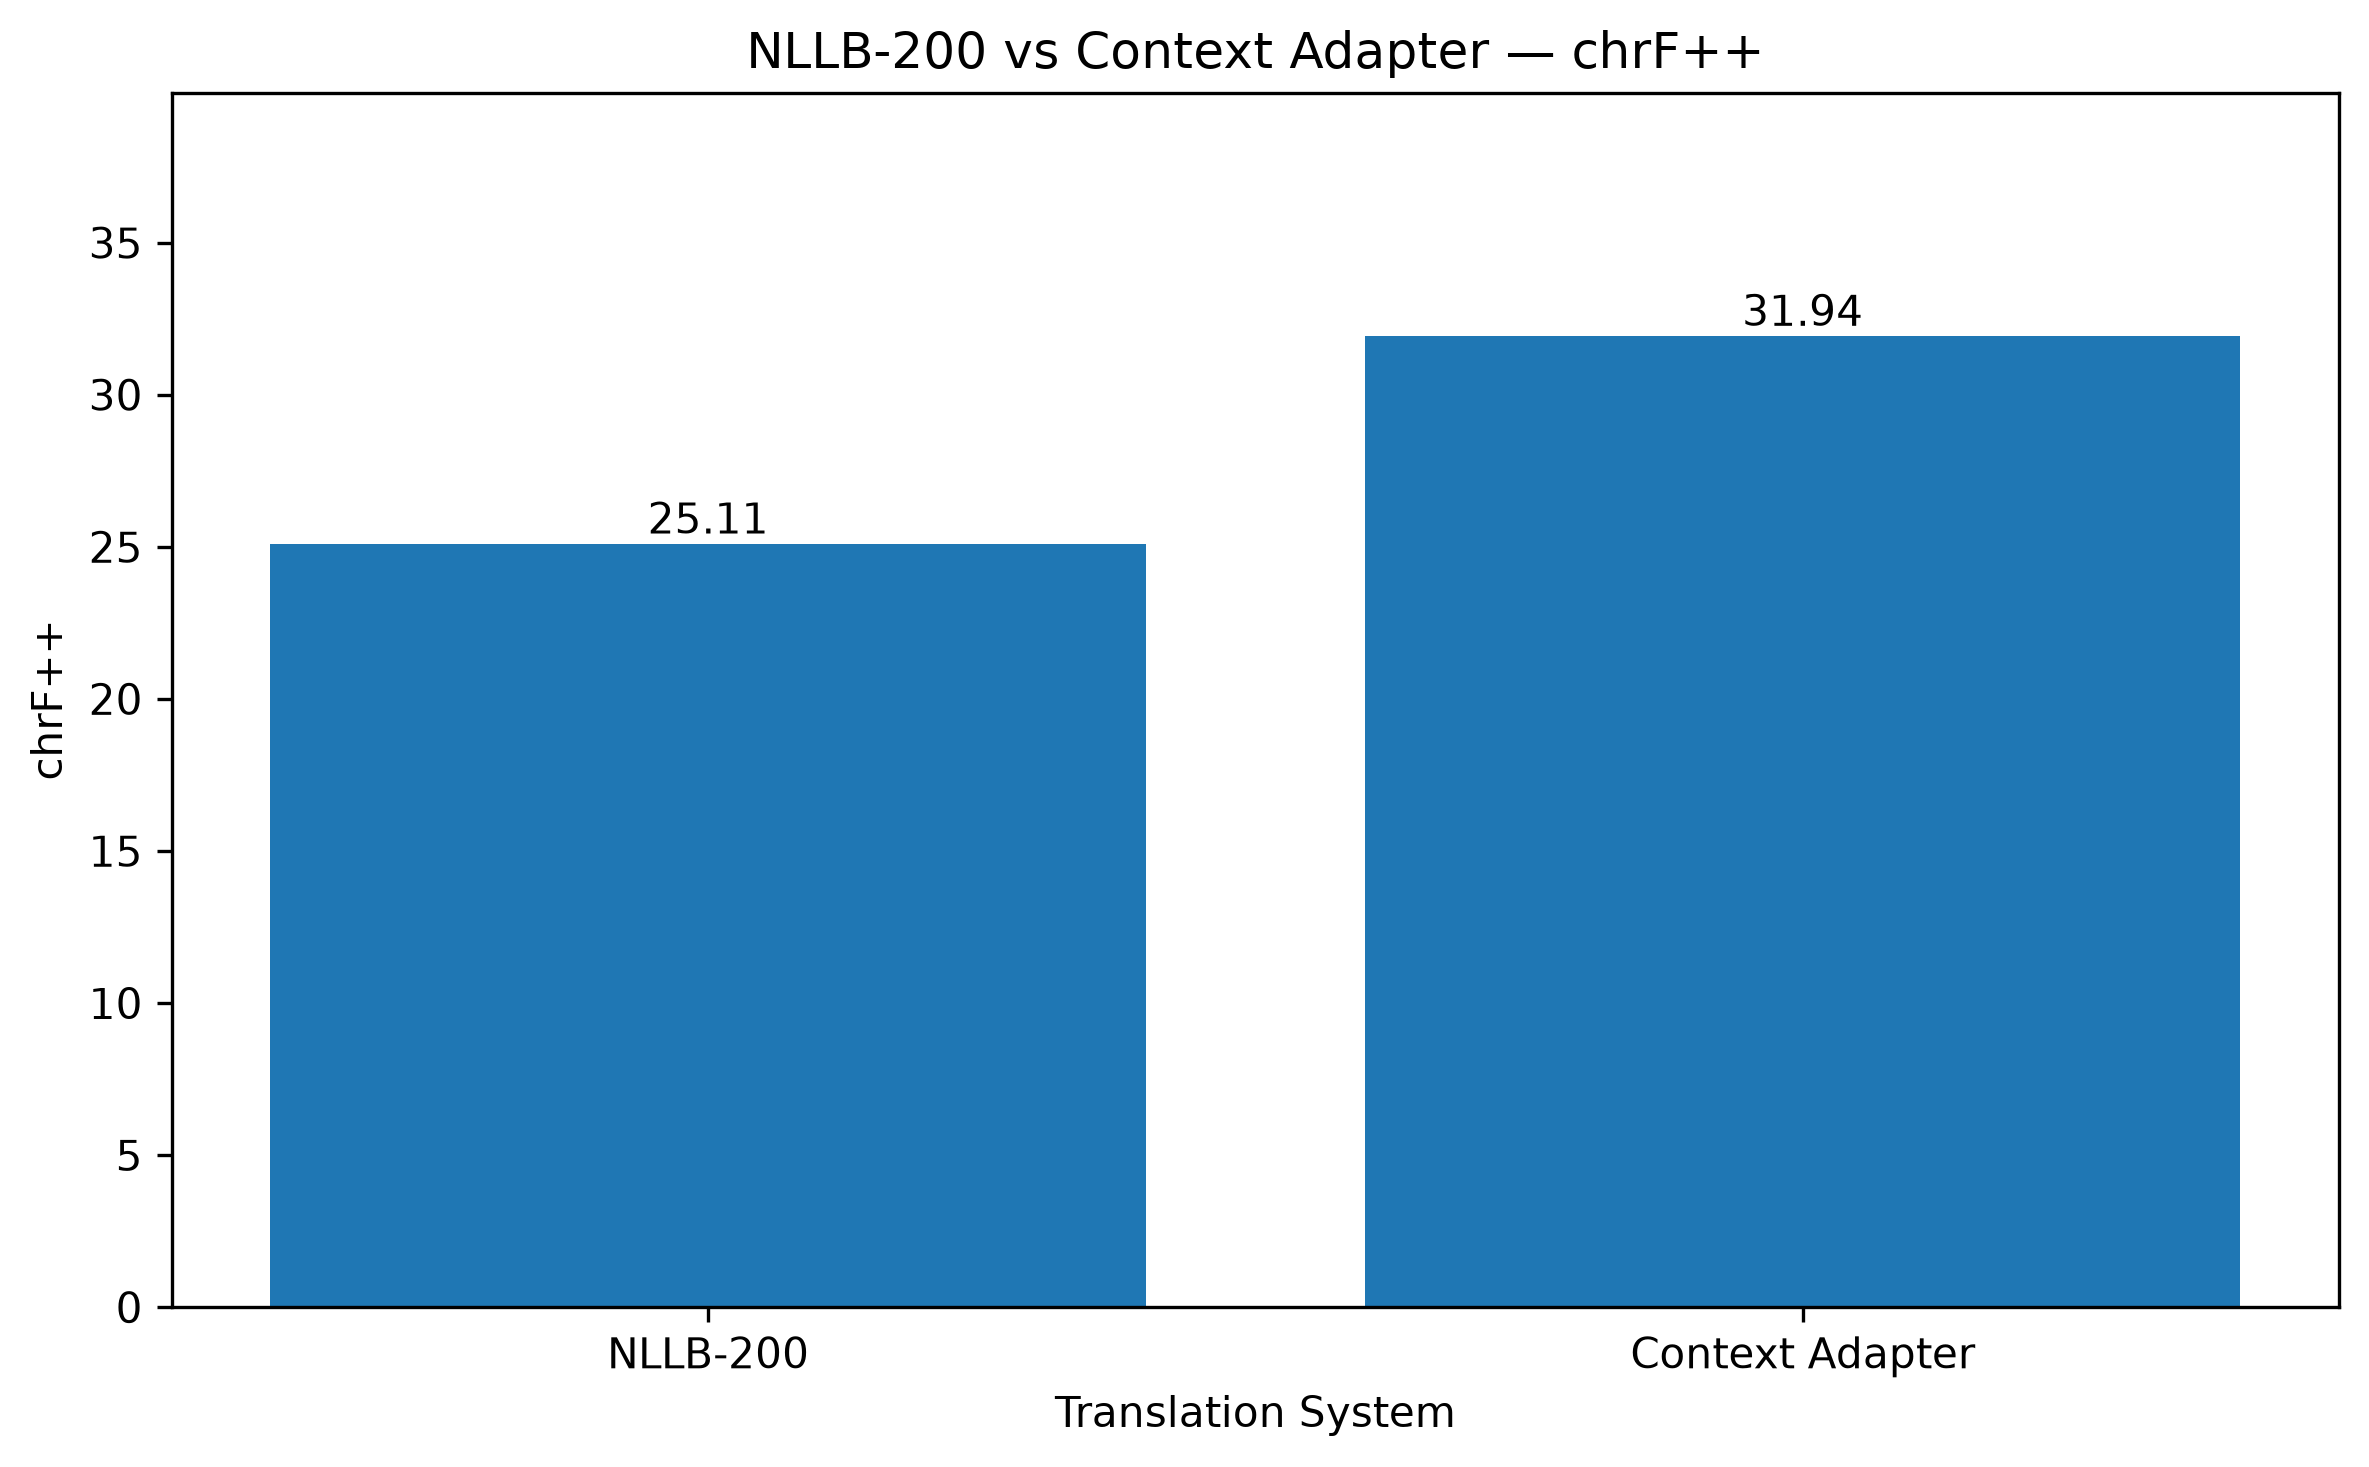
\includegraphics[width=0.82\columnwidth]{figures/final_chrf_comparison.png}
\caption{Corpus chrF++ comparison between the frozen sentence-level NLLB-200 baseline and the proposed Context Adapter on the 100-example validation set.}
\label{fig:chrf_comp}
\end{figure}

\subsection{Comparison with Naive Prefix Concatenation (12-Example Diagnostic)}
To answer \textbf{RQ2} and evaluate whether gated latent fusion is necessary compared to straightforward text concatenation, we analyze a separate, manually reviewed diagnostic subset of 12 document-grounded examples. Table~\ref{tab:diagnostic_prefix} details the comparative metrics.

\begin{table}[ht]
\caption{Diagnostic Comparison: Baseline vs. Naive Prefix vs. Gated Context Adapter (12 Examples)}
\label{tab:diagnostic_prefix}
\centering
\resizebox{\columnwidth}{!}{%
\begin{tabular}{lcccc}
\toprule
\textbf{Configuration} & \textbf{BLEU} & \textbf{chrF++} & \textbf{$\Delta$ vs. Base} & \textbf{$\Delta$ vs. Prefix} \\
\midrule
NLLB Baseline & 41.2778 & 53.4824 & -- & +31.0586 \\
Naive Prefix Concatenation & 10.2193 & 37.0243 & -31.0586 & -- \\
\textbf{Context Adapter (Ours)} & \textbf{43.1483} & \textbf{63.2564} & \textbf{+1.8704} & \textbf{+32.9290} \\
\bottomrule
\end{tabular}%
}
\end{table}

The empirical evidence on this 12-example diagnostic subset reveals a dramatic dichotomy:
\begin{itemize}
    \item \textbf{Catastrophic Prefix Failure:} Concatenating preceding sentences directly into the text prompt (\texttt{CONTEXT: ... CURRENT SENTENCE: ...}) causes performance to collapse by \textbf{-31.06 BLEU} (from 41.28 down to 10.22) and \textbf{-16.46 chrF++}. Inspection of model outputs reveals that the frozen NLLB decoder, having never been pretrained on contextual meta-tags, is confused by prompt formatting and begins translating or repeating the context prefix instead of the target sentence.
    \item \textbf{Gated Adapter Stability:} In sharp contrast, our gated Context Adapter avoids input prompt distortion entirely, maintaining baseline fluency while improving translation to \textbf{43.15 BLEU} (+1.87 over baseline) and \textbf{63.26 chrF++} (+9.77 over baseline).
\end{itemize}

\subsection{Context-Window Diagnostic ($k \in \{0, 1, 2\}$)}
To evaluate \textbf{RQ3}, we examine the influence of context window depth by evaluating the same trained adapter checkpoint across varying context configurations: $k=0$ (empty context vector passed to adapter), $k=1$ (single preceding context sentence), and $k=2$ (two preceding context sentences). Table~\ref{tab:window_diagnostic} and Figure~\ref{fig:window_diag} report these results.

\begin{table}[ht]
\caption{Context-Window Diagnostic Across Context Depths (100 Examples)}
\label{tab:window_diagnostic}
\centering
\resizebox{\columnwidth}{!}{%
\begin{tabular}{lcccc}
\toprule
\textbf{Configuration} & \textbf{BLEU} & \textbf{chrF++} & \textbf{$\Delta$ BLEU vs Base} & \textbf{$\Delta$ chrF++ vs Base} \\
\midrule
NLLB Baseline & 7.3497 & 25.1066 & -- & -- \\
Adapter ($k=0$) & 14.8301 & 28.1975 & +7.4804 & +3.0909 \\
Adapter ($k=1$) & 14.5583 & 31.7309 & +7.2086 & +6.6243 \\
\textbf{Adapter ($k=2$)} & 13.9866 & \textbf{31.9352} & +6.6368 & \textbf{+6.8285} \\
\bottomrule
\end{tabular}%
}
\end{table}

\begin{figure}[htbp]
\centering
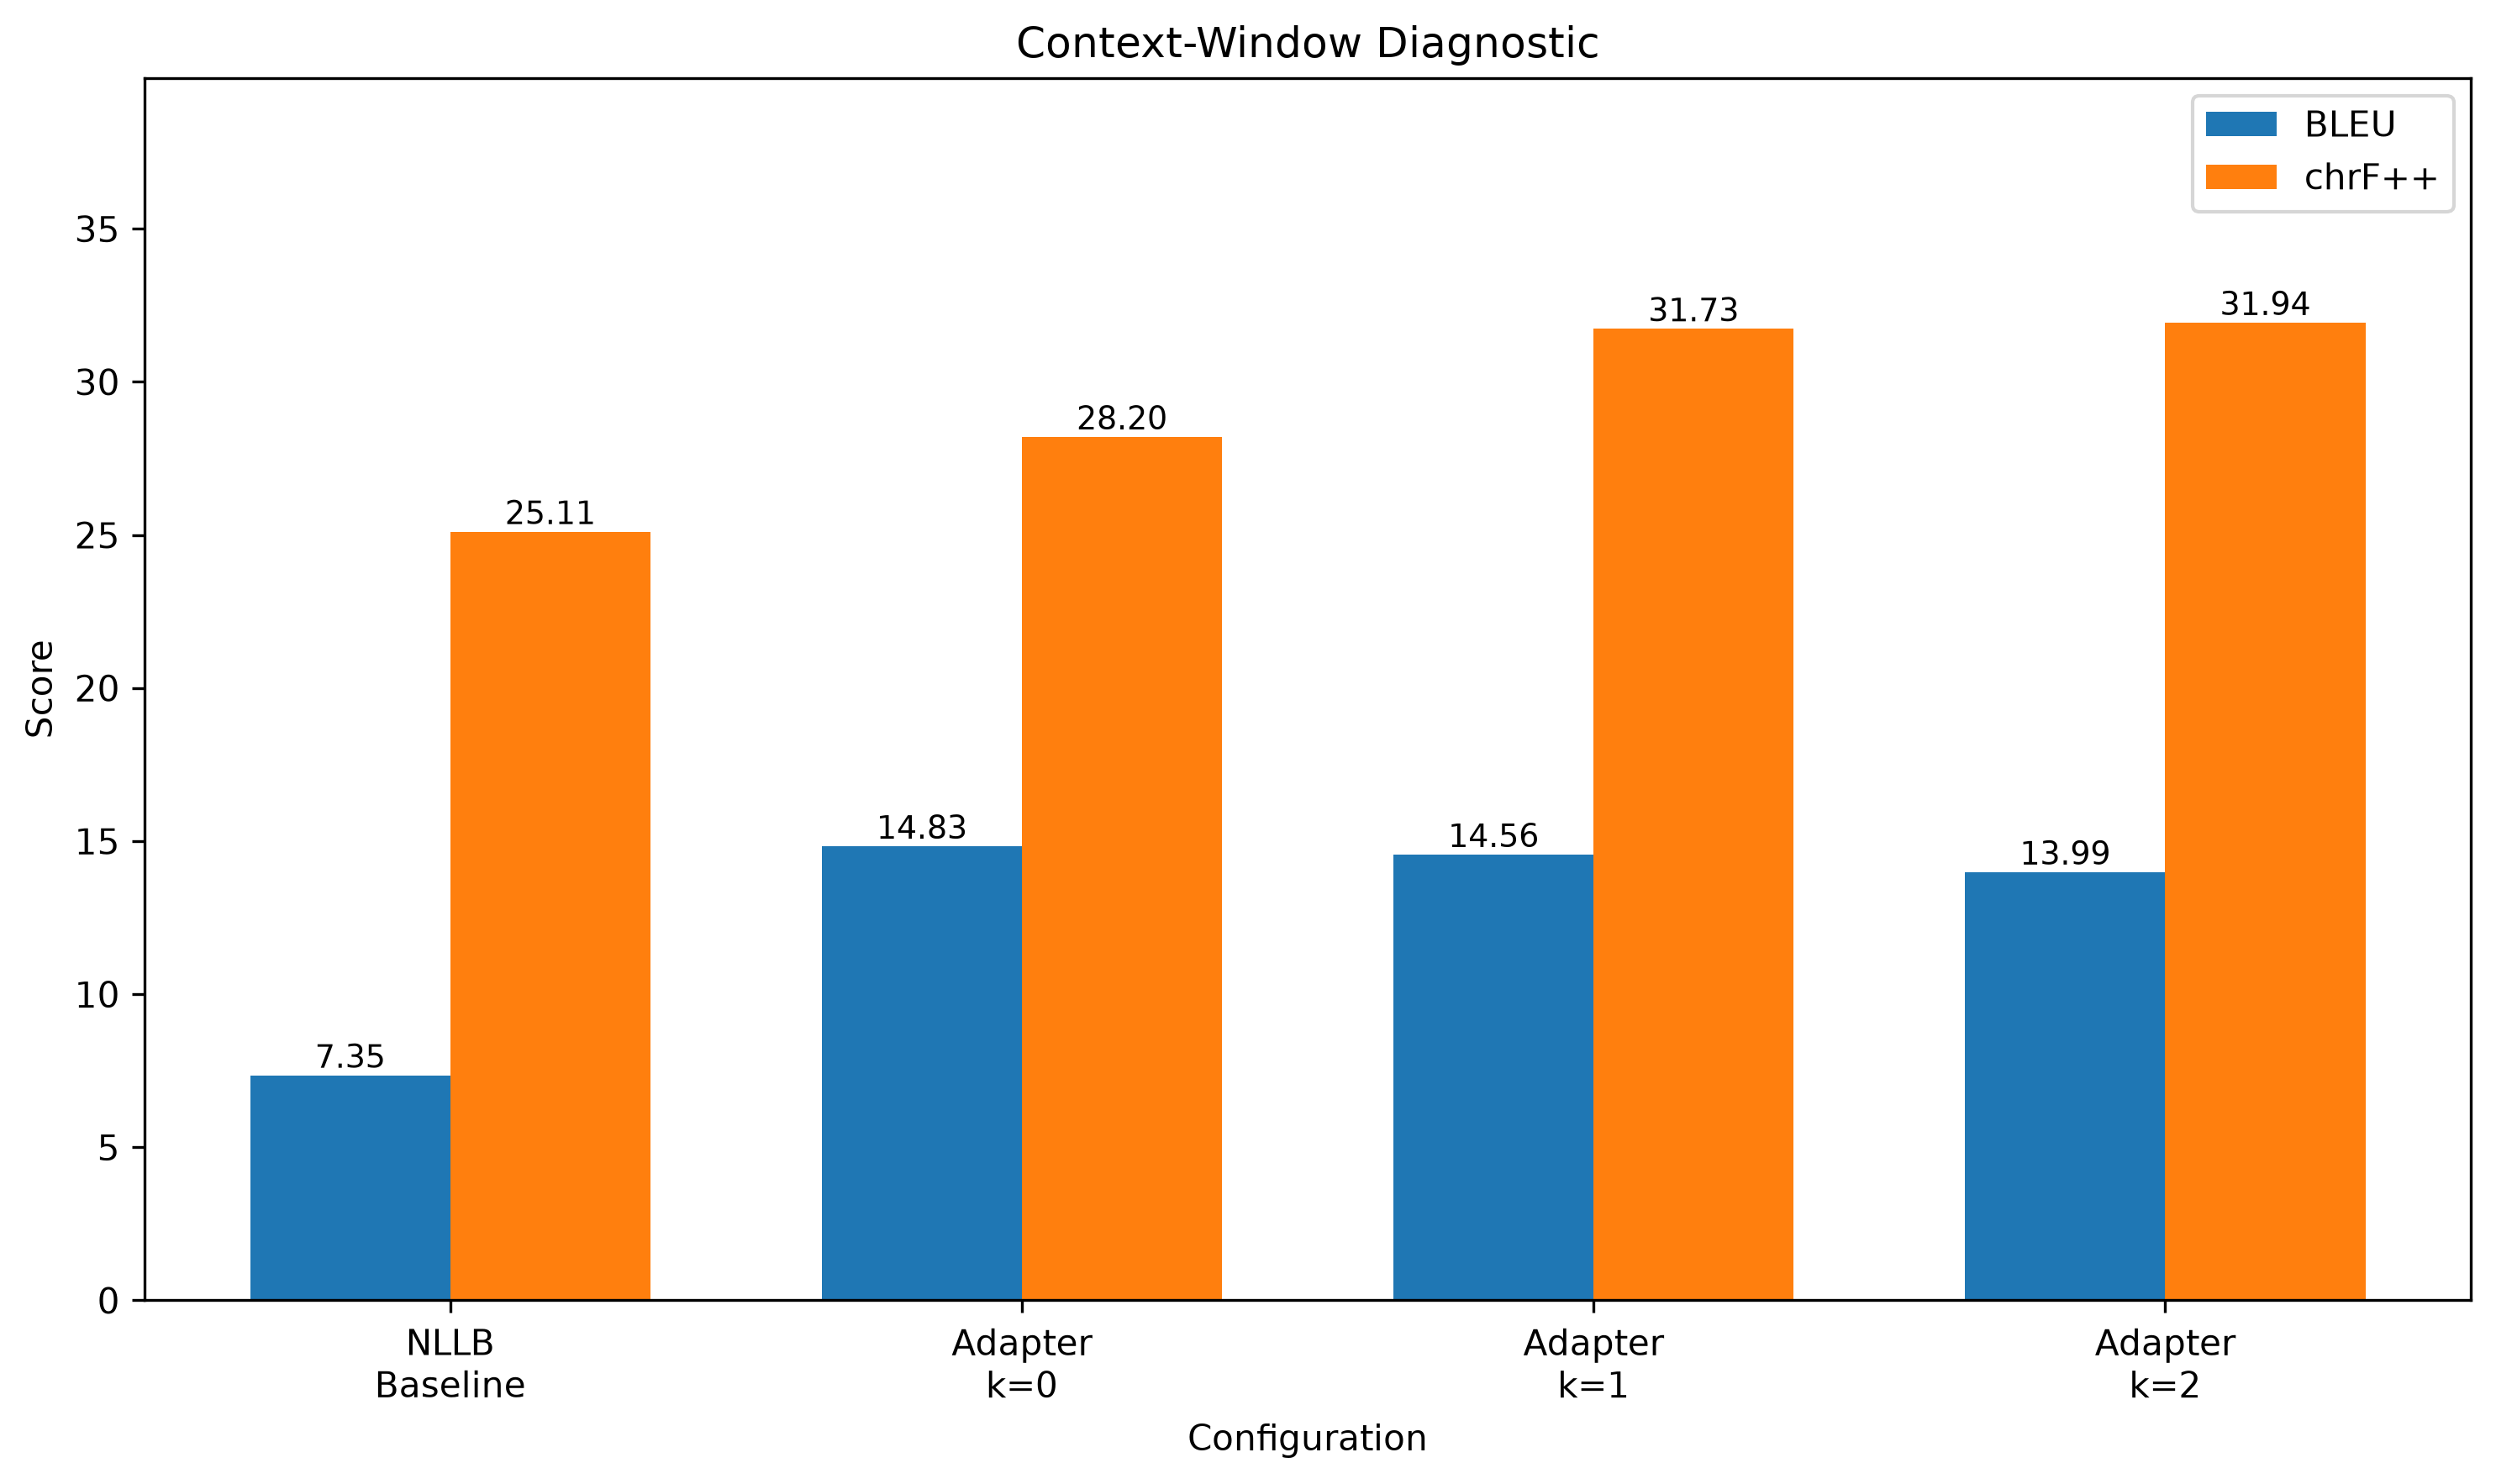
\includegraphics[width=0.92\columnwidth]{figures/context_window_diagnostic.png}
\caption{Performance progression across context window configurations ($k=0, 1, 2$) compared to the frozen sentence-level baseline on the 100-example validation set.}
\label{fig:window_diag}
\end{figure}

\noindent\textbf{Critical Scientific Caveat:} All three settings ($k=0, 1, 2$) utilize the \textit{exact same adapter checkpoint} trained with $k \le 2$. Consequently, this represents an inference-time diagnostic probing rather than three independently trained ablation models. The results indicate that while lexical BLEU peaks at $k=0$ (benefiting from general stylistic adapter shifts), morphological and subword alignment measured by chrF++ increases progressively from 28.20 at $k=0$ to 31.73 at $k=1$ and 31.94 at $k=2$, confirming that multi-sentence historical context systematically enriches target vocabulary coverage.

\subsection{Per-Example Distribution and Win/Loss Analysis}
Corpus-level aggregates can mask underlying heterogeneity. We perform an exhaustive per-sentence analysis across all 100 validation examples, categorizing outcomes into Adapter Wins, Baseline Wins, and Ties based on sentence-level BLEU and chrF++ deltas. Table~\ref{tab:win_distribution} displays the distribution.

\begin{table}[ht]
\caption{Per-Example Win, Loss, and Tie Breakdown (100 Examples)}
\label{tab:win_distribution}
\centering
\resizebox{\columnwidth}{!}{%
\begin{tabular}{lccc}
\toprule
\textbf{Evaluation Metric} & \textbf{Adapter Wins} & \textbf{Baseline Wins} & \textbf{Ties} \\
\midrule
Sentence BLEU & 52 (52.0\%) & 14 (14.0\%) & 34 (34.0\%) \\
Sentence chrF++ & 52 (52.0\%) & 30 (30.0\%) & 18 (18.0\%) \\
\textbf{Both Metrics Concurrently} & \textbf{40 (40.0\%)} & \textbf{10 (10.0\%)} & -- \\
\midrule
Average Sentence-Level $\Delta$ & \multicolumn{2}{c}{BLEU: \textbf{+6.9724}} & chrF++: \textbf{+7.4678} \\
\bottomrule
\end{tabular}%
}
\end{table}

On this 100-example validation subset, the adapter outperforms the baseline on 52\% of sentences in both metrics, while the baseline outperforms the adapter on 14\% (BLEU) and 30\% (chrF++) of sentences. On 40\% of all sentences, the adapter achieves simultaneous improvements in both metrics, compared to 10\% where the baseline wins on both. These sentence-level distributions highlight consistent local improvements on the evaluated subset without asserting statistical significance.

\subsection{Qualitative Analysis and Error Categorization}
To examine translation mechanics, Table~\ref{tab:qualitative} contrasts qualitative examples drawn from our audited validation logs.

\begin{table*}[t]
\caption{Representative Qualitative Examples Illustrating Contextual Wins and Error Modes}
\label{tab:qualitative}
\centering
\small
\begin{tabular}{p{0.18\textwidth}p{0.22\textwidth}p{0.22\textwidth}p{0.28\textwidth}}
\toprule
\textbf{Source Sentence \& Context} & \textbf{Human Reference} & \textbf{NLLB Baseline Output} & \textbf{Context Adapter Output (Ours)} \\
\midrule
\textbf{Win: Entity Preservation}\newline
\textit{Src:} ``Google Chrome''\newline
\textit{Ctx:} [``...click website, e.g. Google.com'', ``Click OK...''] &
Google Chrome\newline
\textit{(Target retains Latin script)} &
\textit{G\=ugul Kr\=om}\newline
\textit{(Transliterated into Telugu script)} &
Google Chrome\newline
\textbf{[Win: +100 BLEU, +100 chrF++]}\newline
\textit{Preserves Latin entity matching reference context.} \\
\midrule
\textbf{Win: Terminology Consistency}\newline
\textit{Src:} ``- Gujarati Horoscope 2022''\newline
\textit{Ctx:} [``- Tamil Horoscope 2022'', ``- Kannada Horoscope 2022''] &
- Gujarati Horoscope 2022 &
- \textit{Gujar\=at\=i R\=a\'sichakram 2022}\newline
\textit{(Over-translated generic astrology term)} &
- Gujarati Horoscope 2022\newline
\textbf{[Win: +81.0 BLEU, +91.2 chrF++]}\newline
\textit{Harmonizes with preceding section headings.} \\
\midrule
\textbf{Failure: English Copy Bias}\newline
\textit{Src:} ``Buy Standard License -- Music Maker...''\newline
\textit{Ctx:} [``...Bonus Graphic Pack...'', ``...Music Maker Theme...''] &
\textit{Pr\=am\=a\d{n}ika license konug\=olu -- sa\.{n}g\=ita\.{m} Maker...}\newline
\textit{(Partially translated into Telugu)} &
\textit{Pr\=am\=a\d{n}ika license konug\=olu sa\.{n}g\=ita tay\=ar\=id\=aru...}\newline
\textit{(Fluent Telugu translation)} &
Buy Standard License Music Maker...\newline
\textbf{[Regression: -9.66 BLEU, -47.6 chrF++]}\newline
\textit{Context trigger copied untranslated English text.} \\
\midrule
\textbf{Failure: Hallucinated Reduplication}\newline
\textit{Src:} ``Telugu man to become President of INC.''\newline
\textit{Ctx:} [``Ananda'', ``Charyulu was the 1st''] &
\textit{Bh\=arata j\=at\=iya Congress ku adhyak\d{s}ata vahin\v{c}ina toli Teluguv\=aru?...} &
\textit{Telugu vyakti Bh\=arata j\=at\=iya Congress adhyak\d{s}u\d{d}ig\=a ennikayy\=aru.} &
Telugu Man to become President of INC. \textit{Bh\=arata j\=at\=iya Congress adhyak\d{s}u\d{d}ig\=a...}\newline
\textbf{[Regression: -8.47 BLEU, -10.8 chrF++]}\newline
\textit{Prefix hallucination and code-mixed duplication.} \\
\bottomrule
\end{tabular}
\end{table*}

\subsubsection{Identified Context Wins}
As demonstrated in Example 1 and Example 2 of Table~\ref{tab:qualitative}, the Context Adapter excels in preserving named entities, technical trademarks, and domain-specific terminology that should remain in standard Latin script. When the surrounding context establishes technical software documentation or standardized catalog headers (e.g., ``Tamil Horoscope 2022'', ``Kannada Horoscope 2022''), the adapter successfully suppresses inappropriate over-translations produced by the baseline (such as translating ``Horoscope'' into Telugu ``\textit{Raasichakram}''), achieving perfect reference fidelity.

\subsubsection{Identified Failure Modes}
A scientifically rigorous assessment must address failure cases:
\begin{enumerate}
    \item \textbf{Copying Interference:} As shown in Example 3, when preceding context sentences contain prominent English commercial jargon (e.g., ``Music Maker''), the adapter occasionally biases the decoder toward copying the source sentence directly in English rather than translating it into Telugu. This results in severe local chrF++ regressions (-47.64 points).
    \item \textbf{Code-Mixed Duplication:} In Example 4, the adapter generates the untranslated English sentence followed immediately by the Telugu translation, creating an unprompted bilingual repetition. This stems from the small training subset (1,000 examples), which has not fully regularized the gating interface against cross-lingual interference.
\end{enumerate}

\section{Discussion}
\label{sec:discussion}

The preliminary experimental findings suggest that parameter-efficient gated encoder-side fusion provides a viable exploration pathway for document-aware NMT in low-resource Indian languages within the limits of the evaluated subsets. 

\subsection{Why Gated Latent Fusion Outperforms Prefix Prompting}
Pretrained sequence-to-sequence language models like NLLB-200 are exceptionally sensitive to distributional shifts in their input format. Injecting textual formatting tags into the input prompt pushes the sequence into an untrained region of the token manifold, resulting in catastrophic translation collapse (-31.06 BLEU). Conversely, by projecting context embeddings directly into the continuous latent space of the encoder, the Context Adapter operates as an inductive bias that modulates attention weights without altering lexical sequence syntax. The near-zero gate initialization ($b_g = -4.0$) acts as a critical stabilizer, preventing divergence during initial backpropagation steps.

\subsection{Computational and Architectural Efficiency}
With only $2.49\text{M}$ trainable parameters, the Context Adapter requires less than 10 megabytes of storage (\texttt{context\_adapter.pt} is 9.98 MB), compared to over 2.4 gigabytes for the NLLB-200 backbone. In deployment, the frozen backbone weights can be shared across multiple specialized adapters (e.g., different domains or language pairs), radically minimizing memory consumption while delivering document-level contextualization.

\section{Limitations and Threats to Validity}
\label{sec:limitations}

In accordance with scholarly rigor, we document several key limitations:
\begin{itemize}
    \item \textbf{Evaluation Scope and Statistical Generalization:} Quantitative evaluations are conducted on a deterministic 100-example validation subset and a separate 12-example diagnostic subset from DocHPLT. While fully auditable and reproducible, these preliminary findings do not claim statistical significance across general distributions, and larger-scale benchmarks across multi-shard corpora are necessary to establish broad generalization.
    \item \textbf{Adapter Training Boundedness:} The Context Adapter was trained for a single epoch over 1,000 examples with batch size 1 on CPU hardware. Extended multi-epoch training on larger document sets may further mitigate the copying bias identified in Section~\ref{sec:results}.
    \item \textbf{Language Pair Specificity:} Empirical evaluation is restricted to English-to-Telugu translation. While Telugu represents a challenging agglutinative case study, cross-lingual generalizability across Indo-Aryan languages (e.g., Hindi, Bengali) remains to be demonstrated.
    \item \textbf{Metric Constraints:} Automatic lexical metrics (BLEU, chrF++) measure n-gram overlap and do not explicitly evaluate discourse-level phenomena such as ellipsis resolution or long-distance gender-honorific agreement. Formal human evaluation by native Telugu linguists is necessary for comprehensive validation.
\end{itemize}

\section{Conclusion and Future Work}
\label{sec:conclusion}

This research investigated a parameter-efficient, context-aware neural machine translation framework designed to augment frozen multilingual backbones with causal document-level conditioning. Rather than modifying internal decoder layers or converting the model into a native document-level architecture, our approach introduces an encoder-side Context Adapter ($2,494,464$ parameters) with learned gating that fuses dense MiniLM context representations directly into NLLB-200 encoder hidden states before cross-attention decoding. On an audited 100-example English--Telugu validation subset from DocHPLT, preliminary findings demonstrate promising improvements, elevating BLEU from 7.35 to 13.99 (+6.64 absolute) and chrF++ from 25.11 to 31.94 (+6.83 absolute). Furthermore, on a separate 12-example diagnostic subset, our latent gating architecture completely circumvents the catastrophic failure (-31.06 BLEU) suffered by naive input prefix concatenation.

Future work will expand this framework along several axes:
\begin{enumerate}
    \item Scaling adapter training across full multi-shard DocHPLT splits with multi-epoch optimization.
    \item Extending the architecture to cross-attention fusion inside decoder layers to explicitly condition target token generation.
    \item Constructing dedicated contrastive discourse challenge test suites for Telugu to quantitatively measure honorific consistency and anaphora resolution.
    \item Adapting the framework to the IndicTrans2 foundation model to benchmark domain-specific Indic architectures.
\end{enumerate}

% If the target conference guidelines dictate student-only authors and moving project supervision to an Acknowledgment section, uncomment the following block and remove the guide from \author:
% \section*{Acknowledgment}
% The authors express their gratitude to project guide Dr.~G.~Narayana, Department of Artificial Intelligence and Machine Learning, Chaitanya Bharathi Institute of Technology (CBIT), Hyderabad, for technical mentorship and guidance throughout this major project.

\bibliographystyle{IEEEtran}
\bibliography{references}

\end{document}
